\begin{figure}
	\begin{subfigure}{0.49\columnwidth}
		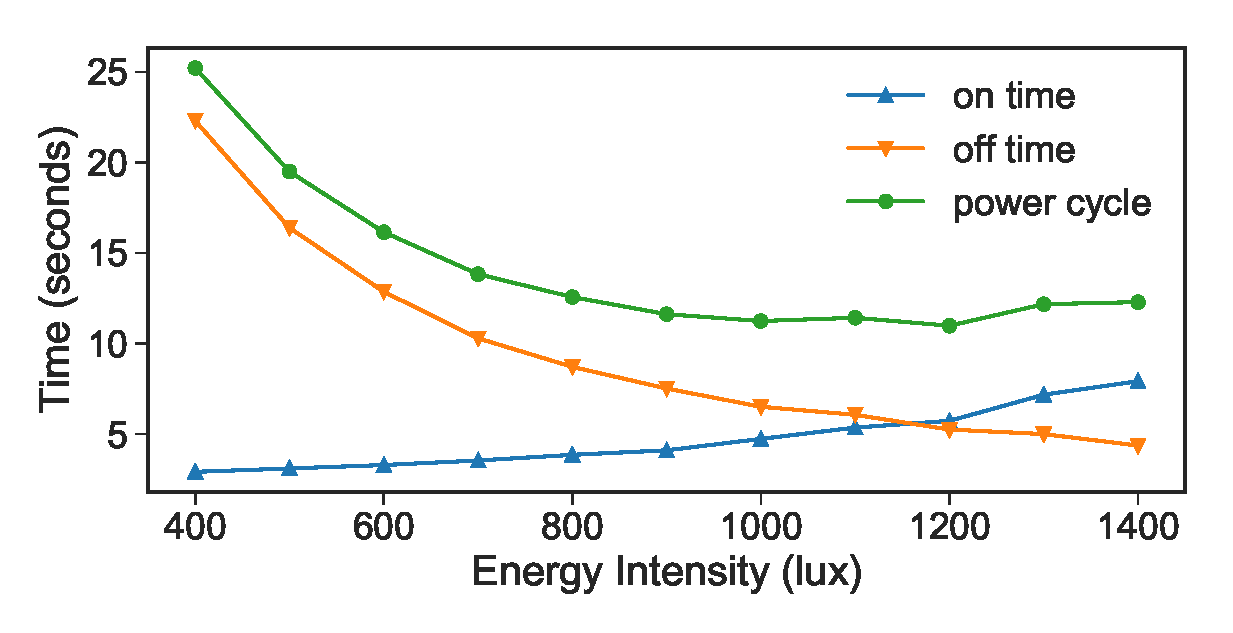
\includegraphics[width=\textwidth]{figures/BatterylessNodesDutyCycles_Sleep_mode}
		\caption{The node powers up and goes into sleep mode. The low energy consumption rate at this mode makes the changes in the on-time when ambient energy changes clearly noticeable. \\  \\ \\ }
		\label{fig:differentEnergyIntensity}
	\end{subfigure}\hfill
	%
	\begin{subfigure}{0.49\columnwidth}
		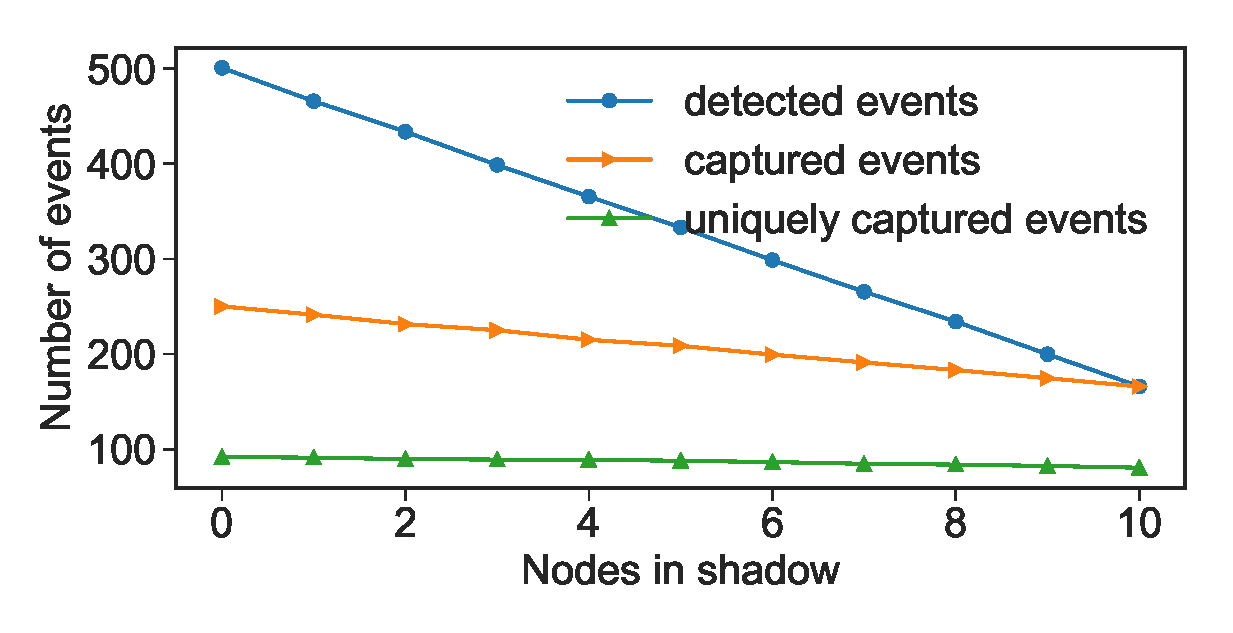
\includegraphics[width=\textwidth]{figures/different_energy_intensity}
		\caption{Simulated results showing how the number of captured events is affected when shadow is covering a \cis. Detected events are \#times events trigger nodes. Captured events are \#times nodes processed events. We used a redundant factor of 2.5 (see (\ref{eq:randFactor}))}.
		\label{fig:sim:differentEnergyIntensity}
	\end{subfigure}
	\vspace{-0.3cm}
	\caption{The effect of non-uniform energy distribution.}
	\label{fig:pwrCycleVSEnergyIntensity}
\end{figure}

\paragraph{Different energy harvesting rates}
It can happen that some of the nodes of a \cis are in the shadow while the rest is under direct sunlight (e.g., when curtains are being opened). 
As a consequence, nodes' power cycles will be significantly different (Figure~\ref{fig:fig:differentEnergyIntensity} shows the on-times, off-times, and power cycles when the ambient energy ranges from 400 to 1400\,lux). Therefore, nodes will not be able to accurately estimate the collective availability of the system. 
%
The inaccurate estimation is most significant when half of the nodes are in shadow. 
However, even during this worst case condition, a \cis availability is not dramatically effected (Figure~\ref{fig:sim:differentEnergyIntensity}). 
This because half of the nodes will overestimate the availability of the system while the other half underestimate the \cis's availability.
During this simulation the power cycles, on-time, and off-time of the nodes are 10, 5, and 5 unit of time when they are under sunlight and 24, 4, and 20 when they are in shadow. 
The length of the simulated experiment is 1000 unit of time.


% Taking into consideration that energy density vary overtime (e.g., the shadow of a curtain moves as the relative position of the curtain to the sun changes), an averaging technique might mitigate the negative effect of non-uniform distribution of ambient energy. However, we believe that these corner cases deserve a deeper and more extended study which is beyond the scope of this work.

\paragraph{Using machine learning algorithms to improve intermittent sensing}
In the future we plan to dive deeper in studying partially captured data. 
Intermittent sensors may partially capture events. Classical recognition 
algorithms face difficulties dealing with partially captured data. 
Therefore, we want to investigate \emph{how much machine learning algorithms 
can improve the sensing quality of intermittent sensing?} 